\documentclass[12pt]{article}
\usepackage{xltxtra}
\usepackage{xunicode}
\usepackage{fontspec}
\usepackage{amsmath}
\usepackage{amssymb}
%\usepackage{verbatim}
\usepackage{fancyvrb}
\usepackage[left=2.54cm,top=2.54cm,right=2.54cm,bottom=2.54cm,nohead]{geometry}
\usepackage{enumerate}
\usepackage{multirow}
\usepackage{array}
\usepackage{graphicx}
\usepackage{url}
\usepackage[
    backend=biber,
    natbib=true,
    style=authoryear-comp,
    alldates=long,
    dateabbrev=false,
    datezeros=false
]{biblatex}
\addbibresource{refs.bib}

\setlength{\parindent}{0pt}
\setlength{\parskip}{1em}

\numberwithin{equation}{subsection}

\bibliography{refs}

\title{Voting simulation: an Eris application}
\date{September 2013}
\author{Jason Rhinelander}

\begin{document}

\maketitle
\thispagestyle{empty}

%\null\vfill
%\begin{center}
%    \copyright 2012 Jason Rhinelander
%\end{center}
%\newpage

% Things I forget:
% A \prec B -- A < B, but with curly <
% A \succ B -- A > B, with curly >
% \precsim, \succsim: same as above, but with ~ below.
% \mathbb{R} -- double-struck R, i.e. rational numbers
% \varnothing -- circle with a line through it, i.e. empty set; also available \emptyset, which uses 0 instead of circle
% \subset, \subseteq, \subsetneq: subset (ambiguous), subset, strict subset
% \superset, ...: same, for supersets
% \dots: ellipsis (...)
% \neg, \AND, \OR: logic symbols for not, and, or
% \iff (alias for \Longleftrightarrow): two-way implication (i.e. two lines in arrow base)
% \Longrightarrow: one-way implication (i.e. two lines in arrow base)
% \cap and \cup for set intersection and union

\section{Introduction}\label{s:intro}

This paper proposes both a modelling technique and preliminary results of an application of that
technique to analyse voting outcomes using richer models than is feasible in the traditional purely
mathematical, equilibrium-based technique.  It accomplishes this through use of the ``Eris''
library, a software library designed by the author for analysing agent-based economic computational
modelling.  The model consists of Downsian-style voters and parties in a one-dimensional issue
space, but several complexities not typically solvable in a mathematical framework: voter movement
through a separate network of friends, and multiple parties with movement constraints.

There are thus three main purposes to this paper: first, as a demonstration and practical
application of the Eris software library; second, as a exploration of how a three-party,
one-dimensional voting system can be modelled; and finally as a demonstration of the
usefulness of agent-based modelling as a technique for exploring economics models.

This model developed in this paper is, in principle, aimed at explaining the existence of fringe,
non-central ideological parties, such as the NDP and the Reform/Canadian Alliance (before merge with
Canada's Progress Conservative party): both parties that have never formed government, yet persist,
despite existing models being unable to convincingly model an equilibrium containing those parties
staying in the fringe.  By allowing for a shifting electorate and constraints on how quickly parties
can move, this paper attempts to provide an explanation for why it might be optimal for such parties
to exist with ideological constraints keeping them out of the center of the political spectrum.

\section{Literature}\label{s:lit}

Agent-based modelling (ABM) and, specifically, its application to economics problems---sometimes
referred to as Agent-based Computational Economics (ACE)---is a technique based on the principal of
emergent behaviour from the complex interaction of relatively simple rules.

One of the earliest works in this technique was the ``Game of Life'', created by mathematician John
Conway in 1970.  Conway's structure consisted of grid points in a two-dimensional space where each
point can be ``alive'' or ``dead'' with simple rules about the number of living neighbours
determining the state of each grid point in the next period\footnote{Specifically, a point continues
living it has 2 or 3 neighbours, comes to life if it has exactly three neighbours, and dies (or
stays dead) otherwise.}.  From these relatively simple rules emerged great complexity over decades
of research; in 2000, Paul Rendell released a Turing machine\footnote{Simply put, a Turing machine
is a system that is theoretically capable of performing any arbitrary computational algorithm}
implemented using only Conway's rules.

In the discipline of economics, the use of computational modelling has gained some traction since
the mid 1990s.  \citet{hce:Tesf} provides an excellent overview of the philosophy and strengths and
weaknesses of ACE.  As she points out, ACE involves specifying less abstract individual behavioural
models than equation-based modelling; the modelling emphasis is on structure rather than equilibrium,
which allows freedoms in modelling that are limited by the assumptions required for ensuring
equilibria in traditional models.  Shes argues that the place for ACE is as a complement, rather
than substitute for mathematical modelling: in this purpose ACE allow us to examine not just the
equilibria of a model, but how---and perhaps more importantly \emph{whether}---equilibria are
attainable.  \citeauthor{hce:Tesf} suggests and warns that programming---which she sees as an
underused but ``beautiful'' branch of mathematics---is insufficiently instructed to economics
graduate students, despite what she sees as the great power of this mathematical approach to
answering the problems of economics.  She concludes aptly that ``programming frees us to adapt the tool to
the problem rather than the problem to the tool,'' recommending an increasing role for teaching
programming skills at the graduate level.

\citet{hce:Judd}, well known for his often-forceful advancement of computational techniques for
economics problems, argues similarly, attempting to address many of the common criticisms of
computational techniques.  \citeauthor{hce:Judd} reinterprets \citet{Tukey62} who, on the topic of
statistical analysis, wrote that ``[t]he most important maxim for data analysis to heed, and one
which many statisticians seem to have shunned, is this: `Far better an approximate answer to the
\emph{right} question, which is often vague, than an \emph{exact} answer to the wrong question,
which can always be made precise.' ''  Judd argues that \citeauthor{Tukey62}'s maxim applies equally
well to economists and computational modelling as it did to statisticians and statistical analysis:
that computational modelling allows analysis of questions that standard models simply cannot
address; rather than shunning such questions economists should embrace computational techniques as a
way to enlarge the set of questions economics can answer.

On the more specific topic of voting models, the literature dates back to at least \citet{Hotelling29}'s
model of single-dimensional spatial competition, which formed the basic foundation of
\citet{Downs57}'s seminal work showing that two-candidate models converge to both candidates
locating at the median voter's position.  \citeauthor{Downs57} goes further, however, in examining
various conditions in which parties do not converge to the median, such as imperfect information of
political parties or voters, shifting tastes of voters, left open the possibility and explored some
richer models using the one-dimensional space by clarifying the various assumptions required.
\citet{Downs57} explores some of these possibilities, concluding that voting models without
strong restrictions can open up many other electoral outcomes other than parties locating at the
median voter.

One of the early works applying ACE to voting models is \citet{KMP92}, which found that parties in
multidimensional issue spaces tend to coalesce to the central regions of the issue space.  The basic
KMP model used in \citet{KMP92} and many later works postulates parties (or candidates) choosing
locations in an $N$-dimensional space, and, unlike in more traditional spatial location models,
imposes constraints on the information they have available while restricting the movements they may
make to a neighbourhood of their current position.  \citet{KMP92}, and most papers following it, use
periodic polling as the only source of the parties' information.  \citet{KMP98} followed up the
earlier paper by looking more closely at the relationship between voter preferences and policy
convergence.  \citet{Plumper08} uses a computational technique involving parties having unlimited
polling ability and an ability to move to any location, but with voter ``memory'' changing the
parties' effective locations to a weighted mean of current and previous positions.  The authors
results show a failure of parties to converge to voter means in multi-party competition in
two-dimensional policy space, but rather to obtain a sort of orbit around, but not at, the
two-dimensional mean.\footnote{
    Earlier work by this author in reproducing the work of \citet{Plumper08} has lead to some doubt
    of the strength of the results of the paper: the few presented ``example'' outcomes in the
    model, upon which much of the paper's conclusions are drawn, appear to be hand-picked examples
    of interesting results rather than typical cases.  Though the paper also included statistical
    analysis concluding that a larger number of parties increased party positioning volatility, that
    analysis was also of questionable quality with likely severe biases because of the construction
    of the data sets used for the analaysis.  More information is available in this author's report
    on reimplementing \citet{Plumper08}, available at
\url{https://imaginary.ca/papers/2013/pm08/report.pdf}.}
\citet{Jackson03} looks at a computational single-dimension, two-party election in which parties
adapt to voters, as in KMP, but voters also adapt their preferences to those of the parties.  An
overview of some of these and other computational approaches to addressing political issues is to be
found in \citet{Handbook29}.

\section{Model}\label{s:model}

The model proposed by this paper consists of a Hotelling-/Downsian-style 1-dimensional voting
space with boundaries at -1 and 1, with negative values considered ``left'' and positive values
considered ``right''.\footnote{The end-points are arbitrary in a
    mathematical sense, but in a computational sense matter: floating point values are stored with
    the same \emph{relative} precision, which means values close to 0 have significantly more
    \emph{absolute} precision than those close to 1.  Making the interval symmetric around 0
    ensures that there is no possible left/right bias coming from numerical imprecision.  Other
    potential ranges (not examined by this paper) are $\hdots, [0.5, 1], [1,2], [2,4], [4,8],
    \hdots$, or subsets thereof, each of which has all values of identical numerical precision.
}  There are a ``large number''---chosen to be 999---of voters distributed in different methods (discussed
below), and a small number (2--4) of parties.  There is also an asymmetric network of voter
friendships that is used to allow voters to influence each other.  Parties get information in each
stage from poll results and use this information to take a step right or left.

Voters in this model have two effects.  First, and most obvious, voters vote for parties and can
observe the party positions.  This paper currently assumes voters are sincere: that is, they vote
for the nearest party.  The second effect of voters is that there is an underlying asymmetric
network of friendships between voters, which is assumed independent of political position.
Asymmetric in this context means that friendships are one-way, i.e.\ $v_A$ can have $v_B$ as a
friend even if $v_B$ does not have $v_A$ as a friend.  This asymmetry could be easily resolved (i.e.\ $v_A$
is a friend of $v_B$ if and only if $v_B$ is a friend of $v_A$), but it is not clear that this would
qualitatively change the result.

The role of friendships in the model is to (temporarily) influence the political position of
friends.  Conceptually, this is capturing a notion that individuals---who make friendships based on
external factors such as office coworkers, familial connections, or neighbourhood proximity---want
their friends to adopt their own beliefs.  Parallels of this in the real world are common in the
political world, where armies of volunteers (who agree strongly with their affiliated party's
political position) attempt to spread their faith in their party to nearby fellow voters.  Another
example is to be found in the devoutly religious, who often receive religious messages as to the
importance of spreading the religious message, e.g.\ spreading ``the word of God.''

Closely related to the model's friendships is a concept of ``voter conviction'', which is a measure
of closeness to the nearest party.  Nearby voters have higher conviction, as they are assumed to
feel more connection with the political system (since there is a party relatively nearby), while
those further away from the nearest party feel more ``left out'' and are thus more apathetic, i.e.\
have lower conviction.  To continue the previous examples, the conviction of a religious
practitioner or political volunteer is thus assumed to be stronger for parishioners or volunteers
closer to that of the religion or party than those whose personal beliefs deviate more strongly.  A
Romney supporter who agrees with all of Romney's policies, for instance, would be expected to be
more passionate in their support of Romney than a voter who votes for Romney only because he is the
marginally closer candidate of two distant options.

Conviction and friendships enter together in how voters influence each other.  At the beginning of
each stage of the model, each voter attempts to influence a random subset of his friends.\footnote{
    The model was also attempted with the alternative formation: each of a random set of voters
    attempts to influence all of his friends.  There was no apparent difference in outcomes between
    the two approaches: each is just a different way of selecting a random set of friendships.
}  If successful, the influenced voter (i.e.\ the friend) changes their position to that of the
influencer; if unsuccessful, the friend doesn't move.  Success is a random outcome, the probability
of which is determined by the convictions of the two voters: voters with high conviction are more
likely to convince friends to move than voters with low conviction; conversely, voters with high
conviction are less likely to be convinced by friend than voters with low conviction.

This procedure alone, however, would result in absorbing states: in each iterations of the game,
more populous regions close to an existing party tend to absorb voters from distant regions, who
then strengthen this absorbing effect until voter distribution converges in probability to a single
point.  To counter this problem, the idea of voter ``drift'' is included in the model: voters are
assumed to have a natural preference at their initial starting position.  When influenced, a voter
jumps to the influencer's location, but then over time drifts back towards their starting location
until they reach it or are
influenced again.

Parties in the model have only limited information on voters, conducted through polling.  In each
period, parties are permitted to take a small, random step in either direction, and may conduct
polls as if the party had taken a step in the previous period.  Thus each party has three sets of
polls: current location, one step up, and one step down, and moves to whichever location yields the
best polling result.

To this model we consider that one of the parties---the one that starts out as the left-most---is
ideologically constrained with a right-most constraint that is 0.1 or 0.2 to the left of the center
of the distribution; of interest in the model results is how (and indeed, whether) this ideological
constraint affects.  This paper also considers what happens when all parties have a ``weak''
constraint imposed, which we define to mean a constraint that allows each party to locate at
the center of the voting space (though some constraints may begin to bind at that point).

The remaining pieces 
An important aspect of voter positions that matters to the model is the concept of voter
``conviction'': voters who are located more closely to the nearest party feel better represented by
the party which, in some sense, validates the voters beliefs.  Voters far away from all parties are
``left out'' and apathetic, i.e. 
that is independent of  Each voter has a fixed set of friends who he
attempts to influence to adopt his own position.   underlying network of friends which
are randomly assigned
(999) of voters and 3 parties The model proceeds in stages involving two types of change: each party of the game Parties can move 


\section{Code}\label{s:code}

\subsection{Eris}\label{s:code:eris}

This project makes extensive use of the open source Eris library, an object-oriented software
library written in the C++ programming language\footnote{Specifically the C++11 specification of the
language.} to serve as a framework for agent-based modelling in general, with a focus on useful
tools for agent-based computational economics in particular.  The Eris source code is publically
available at \url{https://github.com/erisproject/eris}, and API documentation for the project is
publically available at \url{https://imaginary.ca/eris/api}.  Naming conventions used in this
section involve capitalization, such as ``Agent'' or ``Good'', to refer to an Eris progamming
language classes of those name, while lower-case names are used to refer to economic, rather than
programming, concepts.

Eris itself is designed for problems that can be divided into sequential iterations supporting multiple
types of interaction between stages.  The simulation itself consists of programming ``objects''
where each object represents an agent, a market, a good, or set of optimization rules.

For example, consider a very simple microeconomic model consisting of a price-setting monopolist and
many (say 100) consumers, with various utility functions.  In the initial setup of the simulation,
the monopolist would start out with an initial price, consumers would start out with an initial
wealth, and a market object would be created with price and output bundles\footnote{There is no
    intrinsic "money" good in Eris, though one created by convention is often useful; a market's
    price can be measured in any arbitrary good, or even in any combination of goods (e.g.\ a bundle
    of 1 left + 1 right shoes).  Thus general equilibrium exchange economies are perfectly
analyzable using Eris, so long as some exchange mechanism is available.}

In each iteration of the simulation consumers are given a simple choice: optimally spend available
wealth on the monopolist's good.  Since the price is fixed, the decision is a matter of each
consumer choosing a utility-maximizing amount.  This requires, however, a ``Market''
object\footnote{\label{note:mktint}Market is what's called an ``interface'' in object-oriented
    programming: it specifies the programming interface for Market objects, but does not provide the
    actual implementation.  Eris provides two Market implementing classes: Bertrand (where supplies
    offer goods at a given price, with a potential quantity limit), and QMarket (where suppliers
    offer a fixed quantity of goods in each period, and price is determined by (approximate) market
    clearning.).
} in which the consumer can purchase the good from the monopolist, and a \emph{intra-period
optimization} object (``IntraOptimizer'') which attempts to solve the agent's optimization problem.
There are two of these currently included in Eris: ``MUPD'', which relies on the consumer having
differentiable utility and looks at all available markets to equates the marginal utility per money
unit between all of them; and an ``IncrementalBuyer'' object which optimizes by subdividing income
into many small pieces, spending each increment of income on whichever yields the largest increased
in utility.\footnote{In practice, the MUPD approach works much better, but requires that the
    consumer have a closed-form, differentiable, convex utility function.  IncrementalBuyer, on the
    other hand, is a relatively naïve approach that, while putting less requirement on the utility
    function, often fails to obtain an optimal outcome, particularly when there are multiple goods
    available for purchase and those goods are complements or substitutes (since later decisions can
    potentially affect earlier decisions).
}

The monopolist, on the other hand, needs a way to make pricing decisions.  In a very simple example
included in eris, the monopolist makes use of an \emph{inter-period optimization} object
(``InterOptimizer'') which works out a price based on stepping the monopolist's price up or down.
Initially, after the first period, the monopolist has only a single data point consisting of the
number of sales of the previous period, and so can take a step upwards or downwards.  Once the
process repeats a second time, the inter-period optimizer can react by either continuing in the same
direction---if the last change increased profits---or reversing direction---if the last change
decreased profits.  This optimizer also controls the size of the relative price change, taking larger
steps after multiple steps in the same direction (e.g. multiple increases), or reducing the step
size when the reversing direction.

These pieces work together to achieve the same result as a traditional monopoly model after a few
iterations of the simulation (specifically how many depend on individual consumer utilities and
initial monopolist price).  Though not particular interesting on its own, the formulation of the
problem conveys what makes ACE an exciting technique: the model structure only requires specifying
the behaviour of agents and how those agents interact; it does not impose equilibrium, but rather
obtains equilibrium as an \emph{emergent} property of the simulation.  Furthermore it requires no
differentiable market demand function, but instead obtains its outcome through relative simple rules
for the agents programmed into the simulation model.

Extending the same model to a \emph{quantity}-setting monopolist is also possible, but slightly
harder.  It now requires the creation of a considerably more complicated market structure, as
consumer behaviour is still based on market price.  Thus Eris includes a sort of Walrasian actioneer
(called a "WalrasianPricer") that, within a period, tries to get close to the market-clearing price.
This optimization mechanism works by performing a few price ``experiments'' in each round, attempt
to determine the price that just barely exhausts the quantity the monopolist has provided in the
market for a given period.  This complexity is, as in the above case, capable of matching the
traditional quantity-setting monopolist outcome after several periods, though it typically takes
longer (both in terms of number iterations and computational complexity of each iteration) to settle
down because of the complexity added through the pricing experimenting process.

These two examples should, however, be regarded more as benchmarks of the basic building blocks of
the library than useful applications of the library.  While Eris itself provides various useful
functions (the set of which will undoubtedly grow as Eris develops), at its basic level Eris
provides simply a structure in which agent behaviours can be easily programmed and given means to
interact with other agents within and across time periods.

\subsection{Eris application: Voting model}\label{ss:voting}

In creating the voting model analyzed by this paper, much of the machinery described in the examples
above (markets, goods, and prices) can simply be ignored; they are provided, but not required, for
an Eris-based application.  The first step for the voting model was to create a type of agent that
has a position (of arbitrary dimensions) and bounds on that position.  This was added to Eris itself
(rather than specifically to the voting application) as a new type of agent called a
``PositionalAgent'', which simple adds a position property to an Eris Agent's properties.  The
handled position is of arbitrary dimensions, though this voting paper concerns only a
single-dimensional voter and party domain.

There are four types of Agent in this paper's model: ``Voter'' agents, ``Party'' agents, a ``Poll''
agent (which the parties can use to obtain polling information), and an ``FPTP''
(first-past-the-post) agent, which conducts elections.\footnote{Technically there is a fifth type of
    agent called an ``Election'' agent, but like ``Market'' in footnote \ref{note:mktint}, this is a
    programming interface for election-conducting agents.  FPTP is the only current Election agent
    implementation, though others could easily be added without requiring any code changes to the other
    agents.
}  There are also two inter-period optimizer classes: Influence, which governs how Voters exert
influence on their friends, and PartyMover, which slowly shifts Party positions according to polling
data.


Voter agents in this model have a fixed ``natural'' position, which is allocated at
the beginning of the simulation; a ``current'' position, which starts out at the natural position
but can change; a (fixed) set of Voters that are friends; a fixed drift rate; and a conviction
function.  Associated with each voter is an Influence inter-period optimization object which
attempts to exert influence on other voters between periods.  The conviction value of Voters is
defined to be $\max{1 - d_0, 0}$, where $d_0$ is the distance to party nearest the voter.  When a
voter tries to exert influence on a friend, the influence is successful with probability
$\textrm{Pr}(influence) = \frac{1}{2}(1 + c_0 - c_1)$, where $c_0 \in [0,1]$ and $c_1 \in [0,1]$ are the influencer's and influencee's
convictions, respectively.  Thus a voter who is located very close to a party ($c_0 \approx 1$) will
virtually always succeed at influencing a friend who is far away from his nearest party ($c_1
\approx 0$, so $\textrm{Pr}(influence) \approx 1$), while the faraway friend has virtually no chance of convincing
a friend who is very close to a party ($c_0 \approx 0, c_1 \approx 1, \textrm{Pr}(influence) \approx
0$).  Friends of equal conviction have an equal probability of convincing each other.

The initial distribution of voters has (currently) 4 choices: an ``even'' distribution, which spaces
voters perfectly evenly across the voting domain; a ``uniform'' distribution, which draws initial
voter positions from a $\textrm{U}(-1,1)$ distribution; a ``beta22'' distribution option, which
draws from the $\textrm{Beta}(2, 2)$ distribution; and ``beta55'' which draws from the
$\textrm{Beta}(5, 5)$ distribution.  Appendix \ref{app:dists} shows plots and histograms of 999
samples of the 4 distributions.  The number of voters can be configured when running the
application; this paper uses 999 voters in all results.

Party agents have a position and an associated PartyMover optimization object.  Between periods,
this optimization object draws a step of size $s \sim \textrm{U}(10^{-10}, 0.1)$, and is able to
conduct three poll results from the Poll agent: a poll at the ending period's party positions; a
poll where the party considering moving takes a step of $s$; and a poll with the party moving $-s$.
Attempts to move outside the $[-1,1]$ domain are truncated to the domain end-points, though this
doesn't happen in practice.  The party moves to whichever poll yields the highest number of votes.
This polling occurs before any actual movement: that is, each party's poll results do not reflect
any other Party's movement.  Parties are initially distributed evenly across the voting space: in a
2-party model the initial locations would be $\pm\frac{1}{3}$; 3 parties are initially at
$\pm\frac{1}{2}$ and 0, 4 parties are at $\pm \frac 3 5, \pm \frac 1 5$.  Each party can
additionally be constrained to particular location ranges; currently exposed in the program are a $\pm 0.5$
range of each party's initial location, and a specifiable upper range for the left-most party
(i.e.\ the party that starts at the largest, negative location value), so as to allow testing of an
ideologically constrained party.

The Poll agent conducts full population polls, reporting the number of voters who have each party as
a nearest choice.  Parties that are exactly equidistant (which is rare, given the random draw nature
of Party steps) are decided randomly.  Polls are not available in periods where elections occur (see
below).

The FPTP Election Agent is modelled after a first-past-the-post electoral system in which all voters
participate and vote honestly for the nearest party.  The FPTP agent conducts an election every 10
periods in which each agent reports his closest party (deciding ties with a ``coin flip''), and the
winner is the party that receives the most votes (even if not a majority) with ties decided randomly.

The programmed model allows considerable variation in model parameters, as follows (the specific
command options are depicted in Appendix \ref{app:mainhelp}).  Noted values are those used for the
results section of this paper.

\begin{itemize}
    \item Number of parties (from 1 to 10).  This paper considers 3 and 4-party models.
    \item Whether or not parties are constrained to $\pm 0.5$ of their initial location.  This
        paper tests both constrained and unconstrained conditions.
    \item An upper constraint for the left-most (lowest position) party.  This paper tests
        unconstrained, -0.1, and -0.2 values for this parameter.
    \item Number of voters.  This paper uses 999 voters.
    \item Distribution of voters.  This paper uses a $\textrm{Beta}(5, 5)$, which has most voters
        near the center of the voting space.
    \item Number of simulation iterations to run.  This paper uses 1000.
    \item Probability of there being a friendship from any voter to any other voter.  This paper
        uses 0.01 (i.e.\ each voter has, on average, about 10 friends).
    \item The probability that a voter will attempt to exert influence on his friends in a period.
        This paper uses 0.1 (each voter influences about 1 friend per iteration, on average).
    \item Whether the above probability applies to the selection of influencers or influencees.  If
        the former, selected influencers attempt to apply influence to all their friends; if the
        later, all influencers attempt influencing each friend with the given probability.  (Some
        experimentation with this option yielded no discernable difference, and so the results shown
        in this paper used the per-influencee option).
    \item The drift rate for influenced friends (from 0 to 2).  This paper uses 0.05 (an influenced
        voter takes at most 40 time periods to drift back to their natural position).
    \item The length of an election period.  10 was used for this paper.
    \item Whether the election period is periodic (e.g.\ every 10 periods) or random (e.g.\ an
        election randomly occurs with a probability of $\frac{1}{10}$, which yields the same average
        election length).  Randomized elections periods were not attempted for this paper's results.
\end{itemize}

Finally, the simulation provides (optional) output as it runs of the current voter histogram and
party positions, and records winning party information of the simulation to a file.  See Appendix
\ref{app:mainhelp} for detailed command line options, and Appendix \ref{app:output} for an example of the
simulation output.

\section{Results}\label{s:results}

\subsection{Analysis procedure}

To examine the effect of an ideological party, several variations of the model were attempted.
Each variation of the simulation was run for 1000 iterations, consisting of 99 elections at periods
11, 21, etc.  At each election, the winning party and winning party position was recorded.  Each
simulation was run 500 times, each with a different, random seed, and thus covers the same case with
a completely different set of randomly generated values.

Each simulation then has its mean calculated and from these values (500 for each variation) the
mean, standard deviation, and ``5-number summary''\footnote{
    Specifically, min, 1st quartile, median, 3rd quartile, and maximum values.
} were calculated.  For variations where the left-most party has an ideological constraint, the same
values are also calculated for the subset of the data excluding left-most party wins, along with the
proportion of left-most wins.

\subsection{Three parties}

The main case looked at in this model is with three parties in the race, with the following
variations.  Note that in these 3-party cases, the parties start out located at $-0.5, 0, and 0.5$.
\begin{itemize}
    \item No constraints---parties are free to move anywhere in the preference
        domain, most voters start out in the central region.
    \item Party constraints---parties start out at $-0.5, 0, 0.5$ and have weak ideological
        constraints that restrict them to a range of $\pm 0.5$ of their initial location.
    \item Left constraint -0.1---the left party is ideologically constrained to move no more
        rightward than $-0.1$; the other parties are unconstrained.
    \item Left constraint -0.2---the left party is ideologically constrained to move no more
        rightward than $-0.2$; the other parties are unconstrained.
\end{itemize}
The other simulation parameters are as given in section \ref{ss:voting}.

\begin{tabular}{r|r|r|r|r|r|r|r}
    Variation & mean & st.dev. & min & $Q_1$ & median & $Q_3$ & max \\
    \hline
None & -0.000005 & 0.013377 & -0.039527 & -0.009145 &  0.000026 & 0.010024 & 0.036002  \\
All & 0.000063 & 0.010755 & -0.031164 & -0.007685 & -0.000058 & 0.007567 & 0.027739  \\
Left -0.1 & -0.053272 & 0.009673 & -0.078278 & -0.060226 & -0.053907 & -0.047475 & -0.016060  \\
Left -0.2 & -0.043079 & 0.032772 & -0.117607 & -0.067332 & -0.045949 & -0.019134 &  0.057775  \\
\end{tabular}

For the last two cases, results excluding the left-most party are as follows, where the \% column
indicates the mean percentage of time the non-left constrained parties win the election:

\begin{tabular}{r|r|r|r|r|r|r|r|r}
    Variation & \% & mean    & st.dev. &      min & $Q_1$   & median  & $Q_3$   & max \\
    \hline
Left -0.1 & 50.1\% & -0.00296 & 0.02463 & -0.05930 & -0.02145 & -0.00536 & 0.01304 & 0.06754  \\
Left -0.2 & 68.2\% &  0.02850 & 0.01536 & -0.01214 &  0.01910 &  0.02968 & 0.03871 & 0.07401  \\
\end{tabular}


From the results above, it is apparent that ``weak'' ideological constraints on all three parties
have very little effect on the outcome of the elected party: ``None'' and ``All'' have essentially
the same values.  Imposing a strong ideological conditions on one of the parties, however, is able
to induce a notable shift in mean party positions towards that party's position.

Comparing the two tested constraints, -0.1 and -0.2, it is apparent that there are two effects here:
a less ideological party (with a constraint at -0.1) is able to win the election just shy of half
the time (49.9\%), each win pulling the mean winner position to the left, while the party with a -0.2
constraint has considerably fewer electoral victories (31.8\%), but each of those victories pull the
mean elected party position more to the left.  Though not reported in the tables above, it is also worth
noting that the left-most party is almost always at the binding location (-0.1 or -0.2).

Under the left party constraints, the other two parties, on the other hand, take a rightward step in
the voting space, looking for larger vote shares; all of the values in the second table are skewed
considerably to the right.

It thus appears from these results that a non-central, ideologically-constrained party can
effectively stake out a position away from the center, and in doing so, shift the mean electoral
outcome towards itself.  The effect, however, comes about from a more volatile election pattern,
where the winning party jumps periodically from left-constrained to the other two parties, which
generally adopt a right-of-center position.


\subsection{4 parties}

The analysis can easily be extended to see what happens when 4 parties compete in the electoral
system.  The following use identical parameters to the above except for the party positions.  Note
that the ``All'' constraint case has a different interpretation than it does above: where in the
three party case the simulation positions parties such that the two outer parties are able to (just)
reach the center, with 4 parties the equidistant parties are at $-0.6, -0.2, 0.2, 0.6$ with
constraints at $\pm 0.5$.  Thus the two outer parties are effectively both ideologically
constrained: one to the left of -0.1, the other to the left of 0.1.  Though this is an interesting
case on its own, it isn't directly comparable to the above, and so shall only be briefly examined.

\begin{tabular}{r|r|r|r|r|r|r|r}
    Variation & mean & st.dev. & min & $Q_1$ & median & $Q_3$ & max \\
    \hline
None      & -0.000183 & 0.014395 & -0.035579 & -0.010340 &  0.000071 &  0.009696 & 0.040874 \\
All       &  0.000138 & 0.023186 & -0.061240 & -0.017789 & -0.000693 &  0.019191 & 0.059788 \\
Left -0.1 & -0.015990 & 0.011021 & -0.057291 & -0.022813 & -0.016215 & -0.008770 & 0.017735 \\
Left -0.2 & -0.004651 & 0.025723 & -0.080749 & -0.022512 & -0.003261 &  0.013622 & 0.059884 \\
\end{tabular}

The latter two, excluding left-most wins:

\begin{tabular}{r|r|r|r|r|r|r|r|r}
    Variation & \% & mean    & st.dev. &      min & $Q_1$   & median  & $Q_3$   & max \\
    \hline
Left -0.1 & 59.8\% & 0.04456 & 0.01994 & -0.02957 & 0.03186 & 0.04612 & 0.05901 & 0.08538  \\
Left -0.2 & 83.9\% & 0.03221 & 0.01191 & -0.00387 & 0.02466 & 0.03315 & 0.04072 & 0.06254  \\
\end{tabular}

There is still a notable leftward shift, particularly in the weaker (-0.1) ideological constraint,
but it is much less profound than in the 3 party case.  The ideological party still wins far more
than its fair share, at 40.2\% of the time, which helps to pull the mean position leftward.  Like
the three-party case, there is a trade-off in adhering to an ideological constraint: a stronger
ideology results in wins pushing the mean more to the left, but fewer wins cancels out at least some
of this effect.

It is worth noting, in passing, that imposing the dual fringe constraints in the ``All'' condition
(where the two outermost parties can move no closer than 0.1 away from the center) does not
perceptibly change the mean, but does considerably increase the spread of the results.  Closer
analysis of the data reveals that 91\% of elections are won by one of the fringe parties, with the
vast majority of those wins occurring at the binding constraints.


\section{Conclusion}\label{s:conc}

The Eris framework and voting model developed in this paper offers a compelling direction for
research into voting outcomes.  Unlike traditional models, where modelling decisions are often
influenced by mathematical tractability, ACE models in general---and this voting model in
particular---offer a way to ask questions and explore models that go far beyond the capabilities of
traditional models.  Instead of asking ``can model X be solved for an equilibrium'' we can simply
simulate it and see whether an equilibrium emerges.  Our modelling requirements become fundamentally
different: rather than needing to be able to calculating optimal behaviour, we only need to be able
to mathematically specify behaviour.

The results shown above provide an interesting look at one potential ACE model.  One of the driving
forces behind much modern election behaviour is the notion of door-to-door canvassing by armies of
party supporters, aimed not at shifting the party's position, but at shifting voter opinions to be
more closely aligned with the party.  In Canadian politics, the existence of ``left-wing'' and
``right-wing'' parties---such as the New Democrat Party and (pre-merger) Reform/Canadian Alliance
parties has long been a matter that doesn't have a place in a simplified, Downsian-style,
single-dimensional framework.  This model provides a possible answer, in that ideological
constraints may help move the mean electoral result towards the ideological position.  It is,
unfortunately, still hard to draw messages about the real world from the results of such a model,
but this paper serves as a considerable base from which more complicated, more realistic, and more
\emph{real} models can be built to simulate the world around us.


\section{Future Work}

There is a bevy of changes that could be made to the model quite easily to examine how differences
in the behaviour of model agents affects the outcome.  This section summarizes just a few potential
enhancements.  The exciting thing about these suggestions is that most could be easily built into
the Eris voting model developed for this paper, whereas the future work ideas of many papers may run
into tractability problems.  For ACEs, as long as the behaviour can be formalized, the model can be
explored.

Influence could depend not only on the two agents' conviction levels, but also on the
distance between the two agents.  This could capture the intuitive notion that it ought to
be easier for, say, a moderate-left voter located near his party to influence the opinions
of a far-left voter than to influence the opinion of a far-right voters: in other words,
it's easier to convince people to take a small move than a big move, given comparable
conviction levels.

The polling/election system here is very simple: voters simply choose the most preferred
candidate.  Changing this would form the most immediate next step in enhancing this paper.
This would capture the disconnect that is often seen in real-world polling that differs
considerably from actual election outcomes.\footnote{
    For example, recent provincial elections in British Columbia and Alberta have both badly
    mis-predicted election results well outside the bounds of confidence internals that
    sampling statistics should follow.  \citet{ipsos:prebc}, for instance, reports a
    prediction far from the actual results of the following day's election.
    \citet{ipsos:postbc} attempts to justify the corporation's pre-election polls, but does a poor job of
    it, mostly ignoring the likely fundamental issue that poll respondents are simple not a
    good representative of voters.
}  The most complicated part of a polling/election change would be in figuring out the
behaviours that we actually want to capture.  Some interesting poll/election techniques that
would be worth exploring are:
\begin{itemize}
    \item
        Polls here are full-population polls (and thus equivalent to an election where everyone
        participates).  Poll sampling (e.g. choosing a small fraction of voters) might be an
        interesting way to introduce a sort of ``realistic noise'' to the process.
    \item
        Another way to introduce a sort of realistic noise would be to make party distance
        noisy, perhaps by making each party's distance in any period being distributed as
        $d_{perceived} \sim \textrm{N}(d_{actual}, \sigma)$, for some suitable value of
        $\sigma$.  The behavioural analogue would be that it is hard for a voter to tell
        exactly where a party is and that voters typically have only an imprecise view of
        party positions.
    \item
        Voter apathy in the current model is captured (only) in a low conviction value, and
        so has only an indirect political effect through ``social'' consequences (i.e.\ being
        more likely to be convinced by a friend).  Introducing political apathy directly by
        allowing a decision to vote (which could depend on conviction) could easily be
        incorporated; particularly interesting would be to allow such apathy to affect the
        election decision but not the polling decision (i.e.\ polled voters respond with
        their preference to the poll, but don't actually express that preference on election
        day).
    \item
        In reality, electoral behaviour is considerably more complicated that the
        first-past-the-post, true-preference voting explored in this paper:
        voters, especially in a first-past-the-post election system often
        vote strategically.  Some proportion of voters (perhaps inversely proportional to
        conviction) could, for example, use the most recent polling information to choose a
        second-best party to prevent the voter's worst choice from winning.  The polling
        mechanism could be updated to match this intended voting or left as is, so that
        polls are only a rough signal of voter intentions.
    \item
        Other types of election systems could be explored, such as:
        \begin{itemize}
            \item
                coalition governments: a winning party receiving less than half the vote must
                form a coalition with a party to make a combined vote majority, the
                effective government position being a weighted mean of the parties positions
            \item 
                instant runoff voting: if an election doesn't achieve a majority winner, the
                last-place party is removed from the ballot and the election is repeated
                until a majority candidate is chosen.
            \item
                Condorcet voting, where the ordinal party preferences of voters are
                considered to select the party that is most-preferred relative to other
                parties.
        \end{itemize}

\end{itemize}

One area for extension in the political modelling of this paper is to devise more complex political
ideological constraints; instead of a single constrained party matched against two unconstrained
parties, it might also be fascinating to employ the model to examine the effects of having strong
and weak constraint parties on one side of the political spectrum with a weakly constrained party on
the other.  This would allow some insight into the notion of ``vote-splitting'' that is commonly
thought to be a significant factor in Canadian elections: in the 1990s with two competing right-wing
parties and one predominant left-wing party, and the ideologically mirrored late 2000s and 2010s
with two competing left-wing parties and one right-wing party.

The voter friend network could be made dynamic, so that new friendships form and existing
friendships fade, with new friendships being more likely among nearby voters, and lost
friendships being more likely among far off voters.  The model as currently formulated
assumes that friendships are entirely exogenous, but that assumption seems unrealistic.

This model still follows the winner-takes-all approach to government, but there is no fundamental
reason why the model couldn't be made larger to simulate a multi-seat parliamentary election such as
that of Canada.

The results section is only providing a cursory look at the data and as such can find qualitative
but not necessarily quantitative comparisons between the different cases.  Developing a set of
econometric models to analyze the output would certainly be worthwhile.

\newpage

\appendix

\begin{samepage}

\section{Voter Distributions}\label{app:dists}

The following are the available initial voter distributions for the model.  Each graph
shows a histogram of a sample of 999 voters (the value used in this paper) with the
distribution superimposed (except for ``even'', which doesn't have a distribution as such).

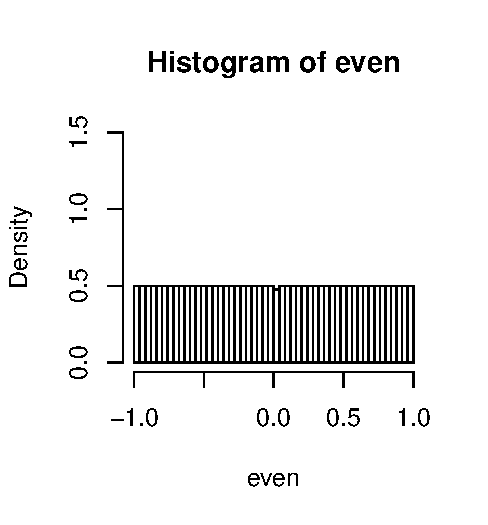
\includegraphics[page=1]{dists.pdf}
\includegraphics[page=2]{dists.pdf}

\includegraphics[page=3]{dists.pdf}
\includegraphics[page=4]{dists.pdf}

\end{samepage}

\section{Voting model invocation}\label{app:mainhelp}

The model is invoked on a command line, with options as shown by the \texttt{--help} command-line
argument, reproduced below.

{\footnotesize\begin{Verbatim}
USAGE: 

   ./main  [-E <v >= 1>] [-e <periodic|random>] [-A] [-D <0.000000 <= v <=
           2.000000>] [-I <0.000000 <= v <= 1.000000>] [-F <0.000000 <= v
           <= 1.000000>] [-H] [-i <v >= 1>] [-d <even|uniform|beta22
           |beta55>] [-v <v >= 1>] [-L <-1.000000 <= v <= 1.000000>] [-c]
           [-p <1 <= v <= 10>] [--] [--version] [-h]


Where: 

   -E <v >= 1>,  --election-period <v >= 1>
     If --election=period: the period of an election.  If
     --election=random: the mean election period length (also the inverse
     election probability).

   -e <periodic|random>,  --election <periodic|random>
     Election type: 'periodic' holds elections at fixed periods; 'random'
     holds an election in each period with a random probability.

   -A,  --influence-all
     If provided, voters attempt to exert influence on their entire set of
     friends at once, with probability given by -I.  The default behaviour
     attempts to exert influence on each voter with the probability given
     by -I.

   -D <0.000000 <= v <= 2.000000>,  --drift-rate <0.000000 <= v <=
      2.000000>
     The speed at which influenced friends drift back to their initial
     location

   -I <0.000000 <= v <= 1.000000>,  --influence-probability <0.000000 <= v
      <= 1.000000>
     The probability that a voter will attempt to exert influence on each
     friend

   -F <0.000000 <= v <= 1.000000>,  --friend-probability <0.000000 <= v <=
      1.000000>
     The probability of any voter being a friend of any other voter

   -H,  --histogram
     Show histogram of voter positions with party positions after each
     iteration.  Requires a terminal supporting/expecting UTF-8 output.

   -i <v >= 1>,  --iterations <v >= 1>
     Number of simulation iterations

   -d <even|uniform|beta22|beta55>,  --voter-distribution <even|uniform
      |beta22|beta55>
     Distribution of voters: 'even' spreads voters evenly over the range;
     'uniform' uses a random uniform distribution; 'beta22' use a beta(2,2)
     distribution; 'beta55' uses a beta(5,5) distribution.

   -v <v >= 1>,  --voters <v >= 1>
     Number of voters to create

   -L <-1.000000 <= v <= 1.000000>,  --constrain-left-below <-1.000000 <= v
      <= 1.000000>
     The upper constraint for the left-most party.  Defaults to 1
     (unconstrained) if parties are not constrained, otherwise defaults to
     the initial party location.

   -c,  --constrained
     Constrain parties to +/- 0.5 of initial location.

   -p <1 <= v <= 10>,  --parties <1 <= v <= 10>
     Number of parties to create

   --,  --ignore_rest
     Ignores the rest of the labeled arguments following this flag.

   --version
     Displays version information and exits.

   -h,  --help
     Displays usage information and exits.


   Eris-based voter/party simulation model
\end{Verbatim}
}

For example, to run the model with a $\textrm{Beta}(2,2)$ voter distribution, a drift parameter of
0.2, 800 voters, 5 parties, elections randomly occurring with a mean of 20 periods, and 2000
iterations in all (with default values for the remaining parameters), and to have a text-based
graphical display of the histogram and party positions, one would use the command:

{\footnotesize\begin{Verbatim}
./main -d beta22 -D 0.2 -v 800 -p 5 -E 20 -e random -i 2000 -H
\end{Verbatim}
}

Election winners and positions would be written to the file
\texttt{results/elections:p5,!c,!L,v800,dbeta22,i2000,F0.01,I0.1,D0.2,!A,erandom,E20,seed=12345.data},
where the seed value is determined randomly (or can be specified by setting the
\texttt{ERIS\_RNG\_SEED} environment variable).


\section{Sample output}\label{app:output}

If run with the \texttt{-H} option (see Appendix \ref{app:mainhelp}), the simulation application
produces a histogram of voter positions and party positions at the end of each iteration.  The
following shows a sample of this output for the specific command given at the end of
Appendix \ref{app:mainhelp}.

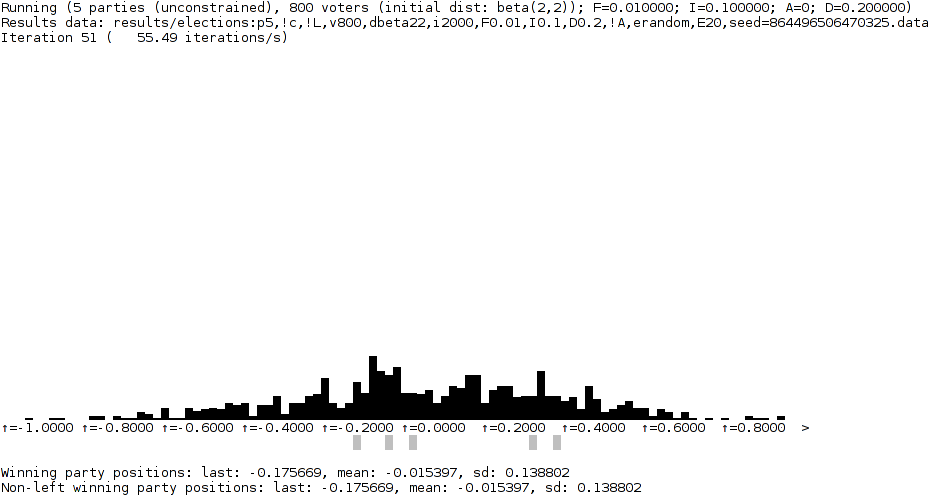
\includegraphics[width=7in]{screenshot.png}


%implementation.
%framework how the library worksmore It should be point
%Optimization objet Eris provides a couple of
%built-in object classes to do this optimization: one which depends on the consumers having
%differentiable utility, which There n optimal have a choice: Consumers would respond to that price
%in making a purchasing decision based on the price and their own rules.  For the next period, the
%monopolist now has the number of sales in the previous period, and can adjust the next period's
%price upward or downward.  After this process repeats again, the monopolist has additional
%information on demand and can use the previous two steps to determine whether to take another price
%change in the same direction, or whether to reverse direction.  This inter-period pricing decision
%is known in Eris teminology as an \emph{inter-period optimization}, the logic for which is contained
%in a dedicated object.
%
%step in th
%downwardFor example, one set of consumer
%behaviour .  Depending on the quantity sold in the period, the
%monopolist could 
%
%The Eris library itself makes extensive use of object-oriented programming, whereby each component
%of a simulation is in an independent ``object'' that has various methods or functions that are
%called to interact with the object.  Eris models are designed to handle sequential time problems,
%where the sequences can b be
%some of the simple
%examples included with Eris, and interlibrary mplements, at its core, a simulation, which itself includes multiple agents, markets,
%goods, intra-period optimizers, and inter-period optimizers.
%

\printbibliography

\end{document}
